\section{Speicher - Custom IP Blocks}
\subsection{Typen von Speicher in FPGA}$~$ \\
In einem FPGA sind normalerweise zwei Arten von Speicher vorhanden:
\begin{compactitem}
    \item \textbf{Distributed Memory}: Distributed Memory besteht aus vielen LUT Tabellen. Der Vorteil dieser Variante ist, dass jede beliebige Grösse von Speicher realisiert werden kann. Desweitern kann dieser Speicher an jedem Ort in einem FPGA erstellt werden. Ideal für kleine Speichergrössen.
    \item \textbf{Block Memory}: Block Memory sind fest implementierte Speicherzellen (Hard IP Block). Diese bestehen aus SRAM Zellen (zwei kreuzgekoppelte Inverter) und sind über das ganze FPGA hinweg verteilt. Oftmals haben sie auch gerade eine Fehlerkorrektur implementiert (bei Xilinx: Hamming Error Correction Code). Ideal für grössere Speichergrössen. Die Speichergrösse bei den Xilinx Series 7 Block Rams beträgt 32kb (36kb physikalisch vorhanden).
\end{compactitem}

\subsubsection{ROM}
ROM wird benutzt um konstante Daten zu speichern. In einem FPGA wird die Implementierung von ROM mithilfe von RAM gemacht.

\subsubsection{Interface Arten}
Beide Speicherarten können mit zwei verschiedenen Schnittstellen implementiert werden.

\begin{minipage}{0.3\textwidth}
    \begin{figure}[H]
        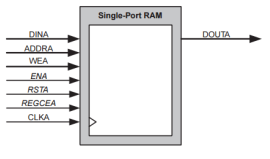
\includegraphics[width=1\textwidth]{images/singleportram.png}
    \end{figure}
\end{minipage}
\hfill
\begin{minipage}{0.65\textwidth}
    \paragraph{Single-Port RAM}$~$ \\
    Single-Port RAM hat einen Daten- und einen Adressbus. Darüber sind sequentielle Lese- und Schreibzugriffe möglich. Wird Distributed Memory verwendet, so ist es auch zusätzlich noch möglich asynchrone Lesezugriffe durchzuführen. \ \\ \ \\ \ \\
\end{minipage}

\begin{minipage}{0.3\textwidth}
    \begin{figure}[H]
        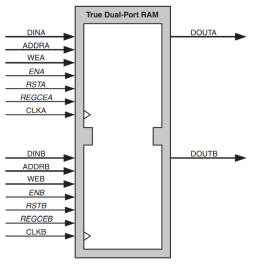
\includegraphics[width=1\textwidth]{images/dualportram.png}
    \end{figure}
\end{minipage}
\hfill
\begin{minipage}{0.65\textwidth}
    \paragraph{Dual-Port RAM}$~$ \\
    Dual-Port RAM erlaubt zwei gleichzeitige Lese- und/oder Schreibzugriffe. Wird über beide Schnittstellen auf die gleiche Speicherzelle zugegriffen, so gibt es eine Arbitrierschaltung, welche diese Situation korrekt abwickelt. \ \\ \ \\ \ \\ \ \\ \ \\ \ \\ \ \\ \ \\ \ \\ \ \\
\end{minipage}


\subsection{Beschreibung von Speicher in VHDL}$~$\\
Es existieren vier Richtlinien für das Beschreiben von ROM und RAM in VHDL. Wird Speicher anhand dieser Richtlinien beschrieben, so sollte der Synthesizer den Speicher korrekt implementieren.
\begin{compactenum}
    \item Die Datengrösse und die Adressengrösse sollen mit generischen Parametern definiert werden.
    \item Der Addressenbereich soll mit einer Konstante definiert werden.
    \item RAM soll mit einem zweidimensionalen Array beschrieben werden.
    \item Der Schreibzugriff muss in einem Prozess beschrieben werden.
\end{compactenum}

\subsubsection{Block RAM - Single-Port}
\lstinputlisting[language=VHDL,style=VHDL]{code/blockram_single.vhd}

\subsubsection{Distributed RAM - Single-Port}
\lstinputlisting[language=VHDL,style=VHDL]{code/distributedram_single.vhd}

\subsubsection{Block RAM - Dual-Port}
\lstinputlisting[language=VHDL,style=VHDL]{code/blockram_dual.vhd}

\subsubsection{ROM}
Da ROM gleich wie RAM implementiert wird, muss nur das RAM Signal als Konstante definiert werden.
\lstinputlisting[language=VHDL,style=VHDL]{code/rom.vhd}

\subsubsection{Synthese-Attribute}
Mit dem Attribut \texttt{ram\_style} kann Vivado mitgeteilt werden, ob das RAM als Distributed RAM (\texttt{"distributed"}) oder als Block RAM (\texttt{"block"}) implementiert werden soll.
\lstinputlisting[language=VHDL,style=VHDL]{code/ram_attribute.vhd}

\subsubsection{Initialisierung}
Eine einfache Art um Speicher zu initialisieren, kann mit Hilfe einer Funktion und einer Datei erreicht werden.
\lstinputlisting[language=VHDL,style=VHDL]{code/rom_init.vhd}

Der Speicher kann aber auch direkt im Code initialisiert werden (eher aufwändig und unübersichtlich):
\lstinputlisting[language=VHDL,style=VHDL]{code/ram_init2.vhd}

\subsection{Memory IP Generators}$~$ \\
Vivado stellt verschiedene IP Generatoren zur Verfügung, über welche direkt Speicher instanziiert werden kann. Diese Generatoren stellen eine einfache Möglichkeit dar, um Speicher nach den eigenen Wünschen zu konfigurieren. Ebenfalls stellen sie präzise Simulationsmodelle zur Verfügung.

\subsection{Intellectual Property IP}
\begin{multicols}{2}
\subsection{Definition IP Core}$~$ \\
Als IP Core (Intellectual Property Core) wird ein vielfach einsetzbarer, vorgefertigter Funktionsblock eines Chipdesigns bezeichnet. Dieser enthält das geistige Eigentum (intellectual property) des Entwicklers oder Herstellers und wird in der Regel lizenziert bzw. hinzugekauft, um es in ein eigenes Design zu integrieren.

\vfill\null
\columnbreak

\subsection{IP Core Typen}
\begin{compactitem}
    \item Hard IP Core: Blackbox in optimierter Layoutform. Sind als fertige Schaltung herstellerseitig unveränderbar in den Chip des FPGAs integriert
    \item Firm IP Core: Synthetisierte Netzliste, die simuliert und wenn nötig geändert werden kann
    \item Soft IP Core: RTL Design. Benutzer muss synthetisieren und layouten
\end{compactitem}
\end{multicols}

\begin{multicols}{2}
\subsection{Bezug von IP Core}
\begin{compactitem}
    \item Ältere bereits vorhandene in-house IP
    \item Neu entwickelte in-house IP
    \item Drittanbieter IP
\end{compactitem}

\vfill\null
\columnbreak

\subsection{Lizenzmodelle}
\begin{compactitem}
    \item Free und Open Source
    \item Kommerzielle Lieferanten (XILINX, CADENCE, ..)
    \item Aggregator (sammelt und kategorisiert IP Cores und verkauft sie weiter)
\end{compactitem}
\end{multicols}

\subsubsection{Konfiguration von IP Blöcken}
\begin{compactitem}
    \item IP Blöcke sind meistens konfigurierbare Module. Jede Instanz eines solchen IP Blocks kann individuell konfiguriert werden.
    \item Konfiguration von Hard IP Blöcken: Beschränkt auf das Ein- und Ausschalten bestimmter Funktionen, da Hardware nicht modifiziert werden kann.
    \item Konfiguration von Soft und Firm IP Blöcken: Flexibler, da diese Blöcke erst nach der Konfiguration synthetisiert werden. Häufig können Funktionalität, Implementierungsstrategie, Schnittstellentyp und Dimensionen eingestellt werden. Konfigurationsparameter werden als generische Parameter an das Modul zur Synthese übergeben.
\end{compactitem}

\subsubsection{IP Packager}
\begin{compactitem}
    \item IP Blöcke bestehen aus vielen Teilen:
    \begin{compactitem}
        \item Quelldateien (RTL, C-Code, Netzlistendateien etc.)
        \item Dokumentation
        \item Simulationsmodelle
        \item Testbenches
        \item Beispiele
    \end{compactitem}
    \item Vivado IP Packager stellt aus obigen Teilen ein Komplettpaket zusammen und legt es in ein zentrales Repositiory (IP Katalog).
    \item IP-XACT: Standard (in XML) für die Verpackung und Dokumentation, welcher von einer Gruppe aus IP-Anbietern unter dem Namen SPIRIT Consortium definiert wurde. Beschreibt nur Schnittstelle und Organisation des Blocks und bietet damit eine Zugangstür für die verschiedenen Werkzeuge, um ihre Informationen zu finden.
    \item component.xml: Enthält Metadaten, Ports, Schnittstellen, Konfigurationsparameter, Dateien und Dokumentation. Ersetzt nicht HDL oder Software (enthält nur High-Level-Informationen).
\end{compactitem}

\subsubsection{Einbinden von IP Blöcken in eigenes Design}
\begin{compactenum}
    \item IP Repository (normalerweise in Projekt oder auf Firmenlaufwerk) dem Projekt bekannt machen.
    \item IP Block aus Katalog auswählen (add IP).
    \item Anpassungen und Generierung spezifischer Ausgabeprodukte (output products): Anpassung erfolgt im IP Integrator. Die Parameter müssen an den RTL-Code des IP Blockes übergeben werden und der Code muss in das Design aufgenommen werden. Bei Generierung der Ausgabeprodukte erzeugt der IP Integrator die kundenspezifischen Designinformationen.
    \item IP verwenden: Der Baustein kann nun verwendet werden, indem er mit dem IP-Integrator im Blockdesign platziert oder in einem herkömmlichen RTL-Design instanziiert wird.
\end{compactenum}
IP Blöcke können verschieden eingebunden werden:
\begin{compactitem}
        \item Via IP Integrator: Vivado führt die folgenden Schritte aus: Instanziierung (Block einfügen in Design), Erzeugung von System-Wrapper (strukturelle VHDL-Top-Level-Beschreibung) und Generierung der Ausgabeprodukte.
        \item Via Instanzierungs-Template im RTL Flow: Für VHDL und Verilog werden Instanzierungs-Templates zur Verfügung gestellt. Der IP Block muss in der Design-Datei, welche eine Position höher in der Design-Hierarchie ist, instanziiert werden.
\end{compactitem}
\lstinputlisting[language=VHDL,style=VHDL]{code/component.vhd}

\subsubsection{IP Life Cycle}
\begin{compactitem}
        \item Vorproduktion (pre-production): IP Core, der öffentlich verwendbar ist, aber noch keine Qualifikationen für den Einsatz in der Produktion aufweist.
        \item Produktion (production): IP Core, der für die allgemeine öffentliche Freigabe zur Verfügung gestellt wird und verifiziert wurde.
        \item Eingestellt (discontinued): Ankündigung von XILINX, dass IP Core bald entfernt wird.
        \item Ersetzt (superseded): IP Core wurde durch eine neuere Version ersetzt.
        \item Entfernt (removed): IP Core wird nicht mehr länger vertrieben.
\end{compactitem}
\begin{tabular}{| l | l | l |}
\hline
\textbf{Change level} & \textbf{User action} & Examples of Changes\\
\hline
Revision & No need to react & Add new device support. Cosmetic GUI changes.\\
 & & Move device support from Pre-Production to Production\\
 & & Extend Parameter range\\
 & & Bug fix for unusable configurations (no working configuration changed)\\
\hline
Minor & May need to react & Reduction in parameter range\\
 & & Remove an optional port\\
 & & Add a memory-mapped register whose use is optional\\
 & & Increased resource usage\\
\hline
Major & Will need to react & Add a non-optional, non-static input port\\
 & & Rename a non-optional port (including case change if Verilog)\\
 & & Change a non-optional port's size\\
 & & Remove a non-optional port\\
 & & Change the interface standard\\
 & & Change or remove a memory-mapped register\\
 & & Behavioral change for all configurations\\
\hline
\end{tabular}
